\section{Diagrama de la solución}

El diagrama de bloques de la solución está recogido en la \autoref{fig:bloques}.

\begin{figure}[h]
    \centering
    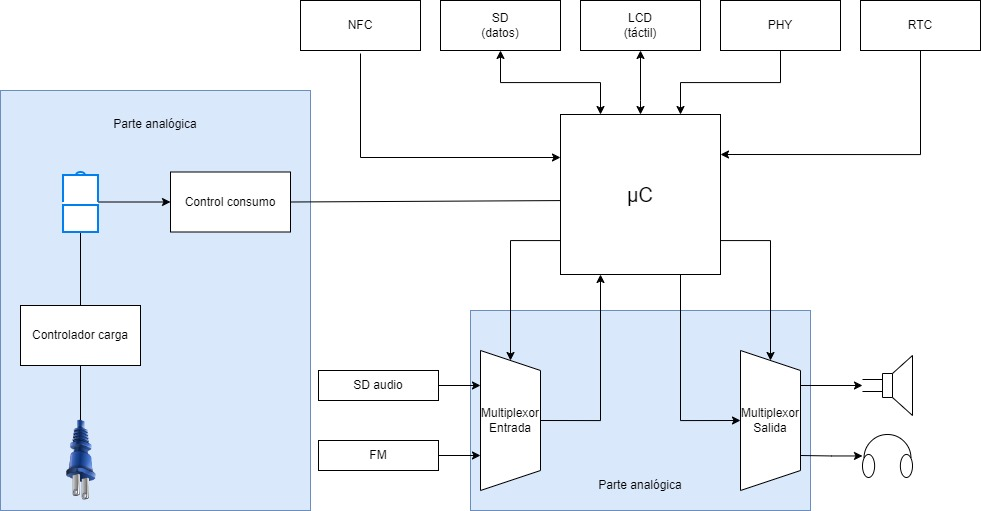
\includegraphics[width=0.75\textwidth]{images/bloques.jpg}
    \caption{Diagrama de bloques de la solución}
    \label{fig:bloques}
\end{figure}

Como se puede ver, el microcontrolador es la parte central del proyecto, conectándose con todos los módulos. Contamos con un módulo analógico de alimentación encargado de cargar la batería y controlar el consumo, y otro también analógico encargado de multiplexar la entrada y salida de audio.

Contamos también con módulos como el sensor NFC, la tarjeta SD para el almacenamiento de datos, el LCD táctil, la interfaz PHY, el RTC interno, el receptor FM o el lector de micro SD para el audio.

El circuito de audio está recogido en la \autoref{fig:audio}.

\begin{figure}[h]
    \centering
    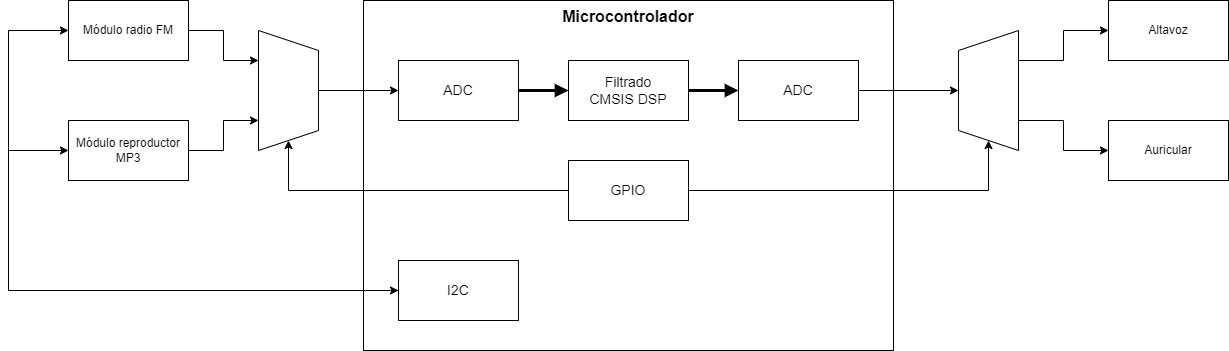
\includegraphics[width=0.75\textwidth]{images/flujoAudio.png}
    \caption{Diagrama de bloques del circuito de audio}
    \label{fig:audio}
\end{figure}

La entrada de audio proviene de un módulo de radio FM o un reproductor MP3 que obtiene las canciones de la tarjeta SD. Ambos módulos ofrecen una salida analógica que se multiplexa hacia la entrada de un ADC del microcontrolador. Los datos digitales atraviesan un módulo software de procesamiento digital de señales basado en CMSIS DSP. El audio procesado se introduce a un ADC, el cual genera la señal analógica de salida. Dicha salida se puede multiplexar entre un altavoz y una salida de auriculares estándar.

Los multiplexores serán controlados con salidas GPIO del microcontrolador.